\section{Conditions aux limites transparentes approximées pour l'équation de dispersion}
\label{sec:TBCKdV}

\indent Dans  \cite{besse2015}, des conditions aux limites transparents exactes sont dérivées pour l'équation de KdV linéarisée (ou équation de Airy) :

\begin{equation}
 	\label{eq:LKdV}
 	u_t + U_1u_x + U_2u_{xxx} = h(t,x), \ \ t \in \mathbb{R}^+, \ \ x \in \mathbb{R}
\end{equation}

\noindent où $U_1 \in \mathbb{R}$, $U_2 \in \mathbb{R}^+_*$ et $h$ est un terme de source.

\indent Pour le problème homogène à valeur initiale

\begin{equation*}
\begin{cases}
	u_t + U_1u_x + U_2u_{xxx} = 0, \ \ t \in \mathbb{R}^+, \ \ x \in [a,b] \\
	u(0,x) = u_0(x), \ \ x \in [a,b] \\
	+ \text{boundary conditions} \nonumber
\end{cases}
\end{equation*}

\noindent les TBCs sont données \cite[équations 2.17,2.18]{besse2015} par 

\begin{equation}
\label{eq:continuousTBC}
\begin{gathered}
        u(t,a) - U_2 \laplinv \left( \frac{\lambda_1(s)^2}{s} \right) * u_x(t,a) - U_2 \laplinv \left( \frac{\lambda_1(s)}{s} \right) * u_{xx}(t,a) = 0 \\ 
        u(t,b) - \laplinv \left( \frac{1}{\lambda_1(s)^2} \right) * u_{xx}(t,b) = 0 \\
        u_x(t,b) - \laplinv \left( \frac{1}{\lambda_1(s)} \right) * u_{xx}(t,b) = 0 
\end{gathered}
\end{equation}

\noindent où $\laplinv$ dénote la transformée inverse de Laplace, $s \in \mathbb{C},\ Re(s)>0$ est la fréquence de Laplace et $\lambda_1$ est, parmi les trois racines du polynôme caractéristique cubique obtenu en résolvant \eqref{eq:LKdV} dans l'espace de Laplace, la seule avec partie réelle négative. \cite{zheng2008}

\indent On a concentré nos efforts dans le cas $U_1 = 0, U_2 = 1$, qui fournit l'équation de KdV linéarisée avec seulement la partie dispersive (qu'on appelle \emph{équation de dispersion}) :

\begin{equation}
	\label{eq:DKdV}
	u_t + u_{xxx} = 0
\end{equation}

\indent Dans ce cas, aussi d'après \cite{zheng2008}, la seule racine avec partie réelle négative est

\begin{equation}
	\label{eq:lambda}
			\lambda(s) = \lambda_1(s) =  -\sqrt[3]{s} 
\end{equation}

\indent Cependant, le calcul des TBCs \eqref{eq:continuousTBC} n'est pas simple en raison des transformées inverses de Laplace, qui donnent à ces conditions un caractère nonlocal en temps. Ainsi, on propose ici des approximations pour la racine \eqref{eq:lambda} qui évitent les intégrations en temps, en générant des TBC considérablement plus simples.

%%%%%%%%%%%%%%%%%% 09/09/2016

\indent Évidemment, comme on va vérifier dans les résultats présentés dans cette section, les TBCs approximées ne sont pas si précises comme les TBCs proposées par \cite{besse2015} (qui les dérive pour la version discrète de l'équation de KdV linéarisée). Néanmoins, en rappelant la discussion initiée dans l'introduction, nos objectifs sont très différents de ceux de \cite{besse2015} : tandis qu'ils cherchent à minimiser l'erreur de la solution calculée (comparée avec la solution analytique) due aux conditions aux bords, on cherche ici à utiliser les TBCs approximées comme conditions aux limites à l'interface (IBCs) dans le contexte d'une méthode de décomposition de domaine (DDM). Ainsi, notre objectif s'appuie sur la convergence de la solution fournie par la DDM à la solution du même problème résolu dans le monodomaine,  indépendamment des erreurs sur les bords extérieurs. 

%\indent Pour dériver nos approximations, on rappele les propriétés suivantes \cite{laplaceTransform} de la transformée de Laplace:
%
%\begin{itemize}
%	\item Linéarité :
%		\begin{equation}
%			\label{eq:linearityLaplace}
%				\laplinv \left[a_1\hat{u}_1(s,x) + a_2\hat{u}_2(s,x)\right] = a_1u_1(t,x) + a_2u_2(t,x)
%		\end{equation}
%	\item Première dérivée : 
%		\begin{equation}
%			\label{eq:firstDerivativeLaplace}
%			\laplinv \left[ s\hat{u}(s,x) \right] = u_t(t,x) + \laplinv \left[ u(0,x) \right] =  u_t(s,t) +  u(0,x) \delta (t)
%		\end{equation}
%	\item Deuxième dérivée : 
%		\begin{equation}
%			\label{eq:secondDerivativeLaplace}
%			\begin{aligned}
%			\laplinv \left[ s^2\hat{u}(s,x) \right] = & u_{tt}(t,x) + \laplinv \left[ su(0,x) + u_{t}(0,x)\right] = \\
%																		   & u_{tt}(s,t) + u(0,x)\delta_t(t) +  u_t(0,x)\delta (t)
%			\end{aligned}
%		\end{equation}
%	\item Convolution :
%	\begin{equation}
%		\label{eq:convolutionLaplace}
%		\laplinv \left[ \hat{u}_1(s,x)\hat{u}_2(s,x)\right] = \laplinv \left[ \hat{u}_1(s,x)\right] * \laplinv \left[ \hat{u}_2(s,x)\right]
%	\end{equation}
%\end{itemize} 
%
%\noindent où $\delta (t)$ est la fonction delta de Dirac et $*$ dénote l'opérateur de convolution.

\indent La linéarité et les propriétés de convolution et des dérivées de la transformée de Laplace  \cite{laplaceTransform} nous motivent à approximer les opérandes des transformées inverses dans \eqref{eq:continuousTBC} par des polynômes dans $s$. Dans les paragraphes suivants, on implémente et test des approximations avec des polynômes constants et des polynômes linéaires.

\subsection{Approximation des TBCs utilisant des polynômes constants}

\indent On utilise le polynôme constant $P_0(s) = c$  pour approximer $\lambda^2/s$. Par ailleurs, en raison de l'expression \eqref{eq:lambda}, on peut approximer les autres opérandes des transformées inverses de Laplace dans \eqref{eq:continuousTBC} uniquement en fonction de $c$ :

\begin{equation}
	\label{eq:appP0}
	\frac{\lambda^2}{s}  = c, \qquad
	\frac{\lambda}{s}  = -c^2, \qquad
	\frac{1}{\lambda(s)^2}  = c^2,\qquad 
	 \frac{1}{\lambda(s)}  = -c 
\end{equation}

\indent En remplaçant \eqref{eq:appP0}  dans \eqref{eq:continuousTBC} et en considérant des approximations différentes pour les bords à gauche et à droite (respectivement avec les coefficients $c_L$ et $c_R$), on obtient les TBC approximées :

\begin{equation}
\label{eq:appTBCP0}
    \begin{gathered}
        \Theta_1^{c_L}(u,x) = u(t,x) - c_L u_x(t,x)  + c_L^2  u_{xx}(t,x) = 0 \\
        \Theta_2^{c_R}(u,x) = u(t,x) - c_R^2  u_{xx}(t,x) = 0 \\
        \Theta_3^{c_R}(u,x) = u_x(t,x) + c_R u_{xx}(t,x)= 0 
    \end{gathered}
\end{equation}

\indent En considérant un domaine discret avec une taille de maille $\Delta x$ et des points $x_0, ..., x_N$ , et en utilisant des approximations par différences finies, les TBCs approximées \eqref{eq:appTBCP0} sont discrétisées comme

\begin{equation*}
    \begin{gathered}
        u_0 - c_L \frac{u_1 - u_0}{\Delta x}  + c_L^2  \frac{u_0 -2u_1 + u_2}{\Delta x^2} = 0 \\
        u_N - c_R^2    \frac{u_N -2u_{N-1} + u_{N-2}}{\Delta x^2} = 0 \\
        \frac{u_N - u_{N-1}}{\Delta x}  + c_R^2    \frac{u_N -2u_{N-1} + u_{N-2}}{\Delta x^2} = 0 
    \end{gathered}
\end{equation*}

\subsubsection{Tests de validation de l'approximation}

\indent Afin de valider nos approximations, observer son comportement général quand on fait varier les coefficients $c_L$ et $c_R$, et comparer nos résultats avec ceux obtenus par \cite{zheng2008} et \cite{besse2015} , on a résolu le même test numérique considéré dans ces papiers : 

\begin{subnumcases}{}
\label{eq:testCaseBesse1}
 u_t + u_{xxx} = 0, \ \ x \in \mathbb{R} \\
 \label{eq:testCaseBesse2}
 u(0,x) = e^{-x^2}, \ \ x \in \mathbb{R}  \\
 \label{eq:testCaseBesse3}
 u \rightarrow 0, \ \ |x| \rightarrow \infty
\end{subnumcases}

\indent La solution fondamentale de \eqref{eq:testCaseBesse1} et la solution exacte du problème  \eqref{eq:testCaseBesse1} - \eqref{eq:testCaseBesse3} sont donnés, respectivement, par

\begin{equation*}
    E(t,x) = \frac{1}{\sqrt[3]{3t}}Ai\left(\frac{x}{\sqrt[3]{3t}} \right), \qquad
    u_{exact}(t,x) = E(t,x) * e^{-x^2}
\end{equation*}

\noindent où $Ai$ est la fonction d'Airy.

\indent En suivant \cite{zheng2008} et \cite{besse2015}, le problème a été résolu dans le domaine spatiale $[-6,-6]$, pour $0 \leq t \leq T_{max}$, avec $T_{max} = 4$. La taille de maille est $\Delta x = 12/500 = 0.024$ et, aussi comme fait \cite{besse2015}, le pas de temps est $\Delta t = 4/2560 = 0.0015625$.

\indent Pour une évaluation quantitative des résultats, on a calculé les mêmes erreurs définies par \cite{besse2015}: pour chaque instant $t_n = n\Delta t$, on définit l'erreur $l^2-$ relative

$$e^n = \frac{\left\Vert u_{exact}^n - u_{computed}^n\right\Vert_2}{\left\Vert u_{exact}^n\right\Vert_2}$$

\noindent et, dans tout l'intervalle de temps, l'erreur maximale $e^n$ et la norme $l^2$ de $e^n$, données respectivement par

\begin{equation*}
 e_{Tm} = \max\limits_{0 < n < T_{max}} (e^n), \qquad
    e_{L2} = \sqrt{ \Delta t \sum_{n=1}^{T_{max}} (e^n)^2 }
\end{equation*}

\indent Afin de vérifier l'influence de $c_L$ et $c_R$ sur les solutions calculées (et, possiblement, identifier des intervalles de valeurs qui donnent les meilleures approximations pour les TBCs), on a fait des tests avec tous les paires possibles $(c_L,c_R) \in \{-10,-1,-0.1,0,0.1,1,10\}^2$. Les résultats ont été classifiées selon leurs erreurs $e_{L2}$ (un critère basé sur l'erreur $e_{Tm}$ fournit un résultat similaire). La figure \ref{fig:firstTestsP0} montre, pour quelques instants, une comparaison entre la solution exacte et les solutions avec la plus grande et la plus petite erreur. Pour nommer la pire solution, on n'a pas considéré les solutions qui n'ont pas convergé (selon le critère arbitraire $e_{L2} > 10$).

\begingroup
\noindent
\begin{minipage}{.5\linewidth}
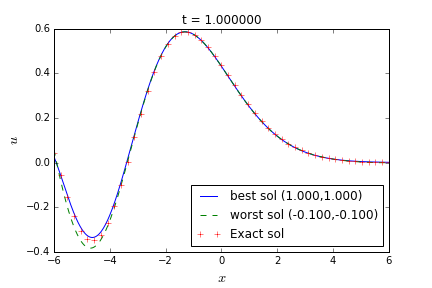
\includegraphics[scale=.5]{figures/BessefirstTestsP0Snap2.png}
\end{minipage}
\begin{minipage}{.5\linewidth}
	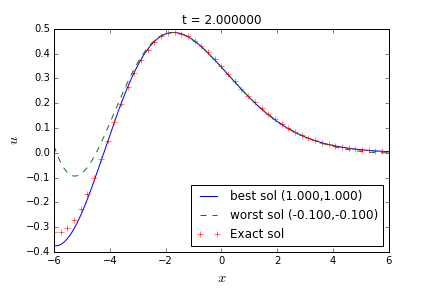
\includegraphics[scale=.5]{figures/BessefirstTestsP0Snap3.png}
\end{minipage}
\begin{minipage}{.5\linewidth}
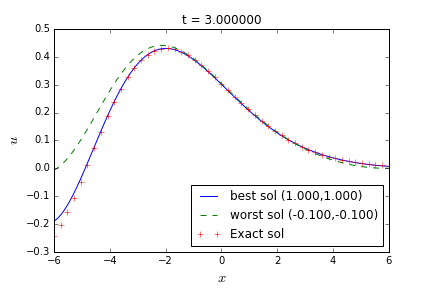
\includegraphics[scale=.5]{figures/BessefirstTestsP0Snap4.png}
\end{minipage}
\begin{minipage}{.5\linewidth}
	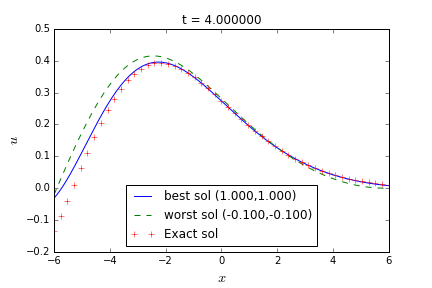
\includegraphics[scale=.5]{figures/BessefirstTestsP0Snap5.png}
\end{minipage}
\captionof{figure}{Meilleur et pire solutions comparées à la solution analytique, dans le cas de l'approximation par un polynôme constant \label{fig:firstTestsP0}}
\endgroup

\indent

\indent Le tableau \ref{tab:firstTestsP0} présente les dix tests avec les erreurs $e_{L2}$ les plus petites :

\sisetup{round-mode=places}
\begin{center}
\begin{tabular}{c|c|S[round-precision=4,table-number-alignment =  left]}
	\multicolumn{1}{c|}{$c_L$}  & \multicolumn{1}{c|}{$c_R$} & \multicolumn{1}{r}{$e_{L2}$} \\
	\hline
	1.0 & 1.0 & 0.0946839239675 \\
	1.0 & 10.0 & 0.097288371204 \\
	1.0 & 0.1 & 0.0983932287563 \\
	1.0 & 0.0 & 0.0992063806502 \\
	1.0 & -10.0 & 0.099359192771 \\
	1.0 & -0.1 & 0.100021589665 \\
	1.0 &  -1. & 0.10159265619 \\
	10.0 & 1.0 & 0.347003021321 \\
	10.0 & 0.1 & 0.347379492262 \\
	10.0 & 0.0 & 0.347487945035
\end{tabular}
\captionof{table}{Meilleurs résultats (les erreurs $e_{L2}$ les plus petites) pour l'approximation par un polynôme constant \label{tab:firstTestsP0}}
\end{center}

\indent On remarque que les résultats sont beaucoup plus sensitives au coefficient pour le bord à gauche : pour un $c_L$ fixé, l'erreur est très similaire pour tout $c_R$. Cela est une conséquence du fait que la solution de ce problème est pratiquement constante et égale à zéro aux voisinages de $x = 6$, mais présente des fortes variations dans la région proche de  $x = -6$. Le meilleur résultat, comme montre la figure \ref{fig:firstTestsP0}, est capable d'imposer ce condition dans le bord à droite, tandis que la pire solution n'en peut pas. Dans le cas du bord à gauche, malgré une erreur plus évidente par rapport à l'autre bord, les meilleures solutions suivent approximativement bien le comportement de la solution exacte.

\subsection{Approximation des TBCs utilisant un polynôme linéaire}

\indent De façon similaire à ce qu'on a fait ci-dessus, on approxime $\lambda^2/s$ par $P_1(s) = ds + c$. Puis, en établissant des relations comme \eqref{eq:appP0}, les convolutions dans \eqref{eq:continuousTBC} s'écrivent :

\begin{equation*}
	\begin{aligned}
    \mathcal{L}^{-1} \left( \frac{\lambda^2}{s}\right) *  u_x(s,x)   =  & \  \mathcal{L}^{-1} \left( \frac{\lambda^2}{s} \hat{u}_x(s,x) \right) =  \mathcal{L}^{-1} \left[ (ds+c) \hat{u}_x(t,s) \right] = \\
    			 & d\mathcal{L}^{-1} \left[ \hat{u}_{xt}(t,s) \right] + c \mathcal{L}^{-1} \left[ \hat{u}_{x}(t,s) \right] = \\
    			 &   du_{xt}(x,t) + du_x(0,x)\delta (t) + cu_x(x,t) \\
    \mathcal{L}^{-1} \left( \frac{\lambda}{s} \right) * u_{xx}(s,x)  = & \   \mathcal{L}^{-1} \left( \frac{\lambda}{s} \hat{u}_{xx}(s,x) \right) =  \mathcal{L}^{-1} \left[ -(ds+c)^2 \hat{u}_{xx}(t,s) \right] =\\
    			&  -d^2u_{xxtt}(x,t) - d^2\delta_t(t) u_xx(0,x) - d^2 \delta(t)u_{xxt}(0,x)  + \\ 
    			& - 2dcu_{xxt}(x,t) -  2dcu_xx(0,x)\delta (t) - c^2u_{xx}(x,t) \\
     \mathcal{L}^{-1} \left( \frac{1}{\lambda^2} \right) * u_{xx}(s,x)  = & \  \mathcal{L}^{-1} \left( \frac{1}{\lambda^2} \hat{u}_{xx}(s,x) \right) = \mathcal{L}^{-1} \left[ (ds+c)^2 \hat{u}_{xx}(t,s) \right] = \\
    			& d^2u_{xxtt}(x,t) + d^2\delta_t(t) u_xx(0,x) + d^2 \delta(t)u_{xxt}(0,x)  + \\
    			& 2dcu_{xxt}(x,t) +  2dcu_xx(0,x)\delta (t) + c^2u_{xx}(x,t) \\
     \mathcal{L}^{-1} \left( \frac{1}{\lambda} \right) u_{xx}(s,x) = & \  \mathcal{L}^{-1} \left( \frac{1}{\lambda} \hat{u}_{xx}(s,x) \right) = \mathcal{L}^{-1} \left[ -(ds+c) \hat{u}_{xx}(t,s) \right] = \\
    			& -du_{xxt}(x,t) - du_{xx}(0,x)\delta (t) - cu_{xx}(x,t)
\end{aligned}
\end{equation*}

\indent En utilisant des différences finies pour les dérivées en temps, et en considérant que la solution initiale est nulle sur les bords (ce qui est le cas de l'exemple testé ici), on obtient les TBC approximées discrètes : 

\begingroup
\footnotesize
\begin{itemize}
 \item \begin{equation*}
\label{eq:appDiscTBCP1}
	\begin{aligned}
    u_0^{n+1} - \left( \frac{d_L}{\Delta t} + c_L \right) \left( \frac{u_1^{n+1} - u_0^{n+1}}{\Delta x}\right) +   \left( \frac{d_L^2}{\Delta t^2} + \frac{2d_Lc_L}{\Delta t} + c_L^2  \right) \left(  \frac{u_0^{n+1} - 2u_1^{n+1} + u_2^{n+1}}{\Delta x^2} \right)  = \\
        -\frac{d_L}{\Delta t}\left( \frac{u_1^{n} - u_0^{n}}{\Delta x}\right) +  \left( 2\frac{d_L^2}{\Delta t^2} + \frac{2d_Lc_L}{\Delta t}\right) \left(  \frac{u_0^{n} - 2u_1^n + u_2^{n}}{\Delta x^2} \right)    -  \frac{d_L^2}{\Delta t^2} \left(  \frac{u_0^{n-1} - 2u_1^{n-1} + u_2^{n-1}}{\Delta x^2} \right)
   \end{aligned}
\end{equation*} 

\item \begin{equation*}
	\begin{aligned}
    u_N^{n+1} - \left( \frac{d_R^2}{\Delta t^2} + \frac{2d_Rc_R}{\Delta t} + c_R^2  \right) \left(  \frac{u_{N}^{n+1} - 2u_{N-1}^{n+1} + u_{N-2}^{n+1}}{\Delta x^2} \right) = \\
     -\left( 2\frac{d_R^2}{\Delta t^2} + \frac{2d_Rc_R}{\Delta t}\right) \left(  \frac{u_N^{n} - 2u_{N-1}^n + u_{N-2}^{n}}{\Delta x^2} \right) + \frac{d_R^2}{\Delta t^2} \left(  \frac{u_N^{n-1} - 2u_{N-1}^{n-1} + u_{N-2}^{n-1}}{\Delta x^2} \right)
    \end{aligned}
\end{equation*} 
   
\item \begin{equation*}
	\begin{aligned}	
    \frac{u_N^{n+1} - u_{N-1}^{n+1}}{\Delta x} + \left( \frac{d_R}{\Delta t} + c_R \right) \left( \frac{u_N^{n+1} -2 u_{N-1}^{n+1} + u_{N-2}^{n+1}}{\Delta x^2}\right) =      \frac{d_R}{\Delta t}\left( \frac{u_{N}^{n} - 2u_{N-1}^{n} + u_{N-2}^n}{\Delta x^2}\right)
    \end{aligned}
\end{equation*}

\end{itemize}

\endgroup

\subsubsection{Tests de validation de l'approximation}

\indent On a répété les tests faites pour l'approximation avec $P_0$, en faisant varier les coefficients $c_L$ et $c_R$ parmi les valeurs dans $\{-10,-1,-0.1,0,0.1,1,10\}$. Afin d'éviter un calcul trop longue, et aussi en utilisant la remarque fait ci-dessus concernant la faible influence des coefficients du bord à droite sur les résultats, tous les tests ont été faits avec $c_R = c_L$ et $d_R = d_L$.

\indent Les dix meilleurs résultats sont présentés dans le tableau \ref{tab:firstTestsP1}. On observe que le meilleur résultat est celui avec $d_L = d_R = 0$ et $c_L = c_R = 1.0 $, ce qui correspond au meilleur résultat parmi les approximations utilisant des polynômes constants.


	 \sisetup{round-mode=places}
\begin{center}
\begin{tabular}{c|c|S[round-precision=4,table-number-alignment =  left]}
	\multicolumn{1}{c|}{$d_L = d_R$}  & \multicolumn{1}{c|}{$c_L = c_R$} & \multicolumn{1}{r}{$e_{L2}$} \\
	\hline
	0. & 1.0 & 0.10754381 \\
	0.1 & 1.0 & 0.14050496 \\
	1.0 & 1.0 & 0.19200976 \\
	10.0 & 0.1 & 0.22789348 \\
	-10.0 & 0.1 & 0.37713227 \\
	10.0 & 1.0 & 0.27161158 \\
	-10.0 &  0.0 & 0.24800816\\
	-10.0 & 1.0 & 0.30039637 \\
	10.0 & 0.0 & 0.27213611 \\
	0.0 & 0.1 & 0.36740764
\end{tabular}
\captionof{table}{Meilleurs résultas (les erreurs $e_{L2}$ les plus petites) dans le cas de l'approximation avec le polynôme linéaire \label{tab:firstTestsP1}}
\end{center}

\subsection{Conclusion partiale}

\indent Il faut être claire que notre approximation ne fournit pas des meilleures TBCs que celles proposées par \cite{besse2015} (et cela n'est pas l' objectif du travail développé ici, comme il a été discuté dans la introduction de ce rapport). En fait, \cite{besse2015} dérive des TBCs pour deux schémas discrets, et le pire résultat parmi eux, en utilisant les mêmes $\Delta t$ et $\Delta x$ utilisés ici, présente une erreur $e_{L2} \approx 0.005$ pour $t = 4$, tandis que notre mieux résultat fournit $e_{L2} \approx 0.1$ pour le même instant. Néanmoins, en considérant qu'on souhaite appliquer les TBCs à une méthode de décomposition de domaine, on veut plutôt minimiser l'erreur due aux conditions limites à l'interface, mais pas l'erreur liée aux conditions aux limites extérieures.

\indent Cependant, en considérant les résultats présentés jusqu'ici, on peut dire que les conditions aux limites proposées simulent relativement bien des TBCs, avec une implémentation assez simple, en comparaison avec celles proposées par \cite{besse2015} (qui demandent par exemple le calcul de $\mathcal{Z}$-transformées, dans le rôle de versions discrètes des transformées de Laplace). Par ailleurs, on remarque que l'approximation qu'on a fait avec le polynôme linéaire, malgré l'augmentation de la complexité du schéma (où il faut garder la solution deux pas précédentes en plus), ne fournit pas des meilleures résultats par rapport au cas du polynôme constant.

\indent Ainsi, dans la suite de notre travail, on a utilisé toujours l'approximation avec $P_0$. On note les TBCs correspondantes avec les opérateurs $\theta_i^c, \ i=1,2,3$, définis dans \eqref{eq:appTBCP0}.

\begin{equation*}
    \begin{gathered}
        \Theta_1^{c_L}(u,x) = u(t,x) - c_L u_x(t,x)  + c_L^2  u_{xx}(t,x) \\
        \Theta_2^{c_R}(u,x) =  u(t,x) - c_R^2    u_{xx}(t,x)\\
        \Theta_3^{c_R} (u,x)= u_x(t,x) + c_R u_{xx}(t,x) 
    \end{gathered}
\end{equation*}